\documentclass[11pt, twocolumn]{article}
\usepackage{microtype}
\usepackage{caption}
\usepackage{subcaption}
\usepackage{graphicx}
\usepackage{subcaption}
\usepackage{mwe}
\begin{document}

\title{Clustering for neuron networks\\using the activation vectors of data}

\author{Zhenge Zhao}

\maketitle

\section{Introduction}

Recent technical developments in the machine learning field have led to huge accuracy increase in a lot of practical applications and research areas such as image classification and pattern recognition. Among these techniques, neural networks are often considered to be the best-performing model and achieve success in many scenarios. However, unlike the previous methods like support vector machine(SVM) or decision tree. The multi-layer structure and the automatic differentiation process turn the neural network into a ``black box". Their results are hard to interpret and the training process is hard to debug.

In addition to that, the nature of the complexity of neural networks also makes comparing them a non-trivial task. Given two neuron networks of different layouts, making direct comparisons is problematic because the difficulties of aligning neurons of different sizes and  matching different dimensions. Moreover, even these two neuron networks are of the same structure but just different initializations or permutations of training batches, the comparison is still nontrivial because high dimensional parameters(e.g. weight and bias) in each layer.

In this project, we propose a new way of clustering neurons networks. Instead of directly comparing neuron networks of different similar structures, we are focusing on the activation vectors produced by neural networks and trying to find neuron networks which treat the dataset in a similar way. In another word, we would like to measure the similarities of two neuron networks by measuring the similarities of data clusters they
produce individually for the same dataset under the same clustering method. We believe this could give us a method of clustering different neuron networks while bypassing the perplexing structures of them.

\section{One sentence description}

We are trying to cluster neuron networks having the same behaviors by using the activation vectors of the data.

\section{Audience for this project}

The outcomes of this project could be very interesting to the machine learning community and model designers. it could help them understand different behaviors of the neuron networks and analyze the models they are constructing. Without adopting such a method, the neuron network will remain to be a ``black box"  while comparing and summarizing the common features of them will be difficult.

\section{Approach Pipeline and technical details}

The core of our approach is generating similarity measurements between two neural network models. Directly comparing structures of those complicated model parameters like weight  and bias of each neuron is hard because of the alignment issue and non-linearities within the hidden layers. The method we propose, however, is suitable for all kinds of model structures as long as we are using the same dataset for the same classification tasks. My method is based on the assumption that the more similar two neuron networks are, they will also cluster the data in a similar way.  Moreover, the activation vectors generated by neural network model for each data point automatically provide a dimension reduction mapping the whole dataset to a feature space which data points are still comparable.

To this end, our approach follows the pipeline below:
\begin{itemize}
	\item Collect the activation vectors for each layer for all instances for each model.
	\item Generate clusters of the dataset for each model by using activation vectors. 
	\item Utilize the cluster structure as representation of the model to calculate the similarity between two models.
\end{itemize}


\subsection{Data collection}
$PyTorch$~\cite{paszke2017automatic} is a well-known library for training neural networks.  We use it to generate 6 models for \emph{Fashion-MNIST} dataset. \emph{Fashion-MNIST} is a dataset of Zalando's article images—consisting of a training set of $60,000$ examples and a test set of $10,000$ examples. Each example is a $28 \times 28$ grayscale image, associated with a label from $10$ classes. We choose a sample of $1000$ including all of the $10$ classes. The 6 models come from two different structures and they differs in \emph{learning rate, momentum or different initializations}. All the 6 models reach an accuracy over $90\%$ and is trained over $100$ epochs.

We stored activations of all the $1000$ data points for all the hidden layers of this 6 models  across every epoch in the local disk for future use. We think the activations generated by hidden layers could collaborate with more information comparing to the single prediction. An the activation vectors of instances are comparable within any epoch of any model since the dimension are automatically matched.

\subsection{Cluster Generation}
For a specific model state(i.e. a epoch for any model), to generate clusters for the $1000$ samples, we could choose a layer of activations therefore each vector have the same dimension $m$ and could represent the corresponding data point.  we use K-means~\cite{macqueen1967} as our clustering approach. Before clustering these vectors, we also apply a dimension reduction method to the vectors since K-means may struggle for high dimensional data. We choose PCA~\cite{jolliffe86} other than TSNE~\cite{vanDerMaaten2008} since it is much faster.

After reducing the dimension of the data, we applied the K-means algorithm with 10 initial clusters. We choose K-means since the number of the clusters can be set as the same as the number of the classes and it has been implemented in the ~\emph{Python} library ~\emph{scikit-learn}. Later, for each cluster, we choose the majority of the true labels within the cluster as the label for this whole cluster.  

\subsection{Model Comparison}
We can choose a pair of models for further comparisons. For each model, we can represent each sample using the representative label of cluster it belongs.
We can then compare two different clusterings by Rand index~\cite{Hubert1985}, which is regular measure of the similarity between two data clusterings in statistics. The Rand index has a value between 0 and 1, with 0 indicating that the two data clusterings do not agree on any pair of points and 1 indicating that the data clusterings are exactly the same. Such a method can represent a model state using the dataset while bypass aligning different dimensions of activation vectors directly.



\section{Visual Analysis}

    \begin{figure*}
	\centering
	\begin{subfigure}[b]{0.475\textwidth}
		\centering
		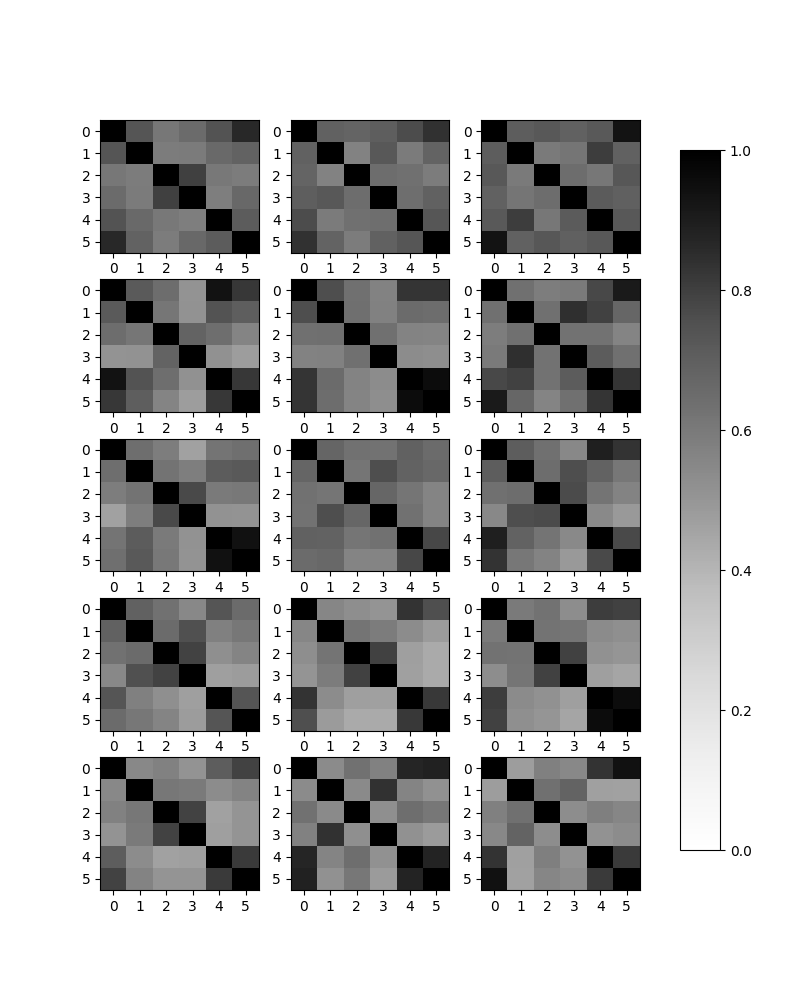
\includegraphics[width=\textwidth]{figs/c1.png}
		\caption[]%
		{{\small First Convolution Layer}}    
		\label{fig:c1}
	\end{subfigure}
	\hfill
	\begin{subfigure}[b]{0.475\textwidth}  
		\centering 
		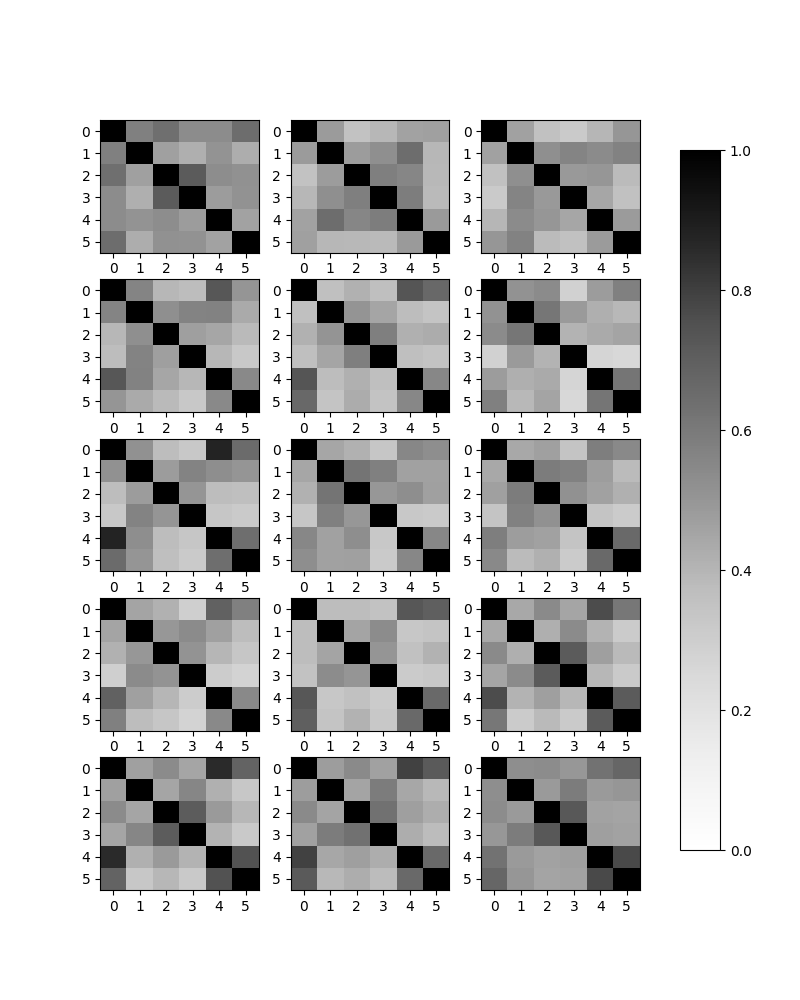
\includegraphics[width=\textwidth]{figs/c2.png}
		\caption[]%
		{{\small First Convolution Layer}}    
		\label{fig:c2}
	\end{subfigure}
	\vskip\baselineskip
	\begin{subfigure}[b]{0.475\textwidth}   
		\centering 
		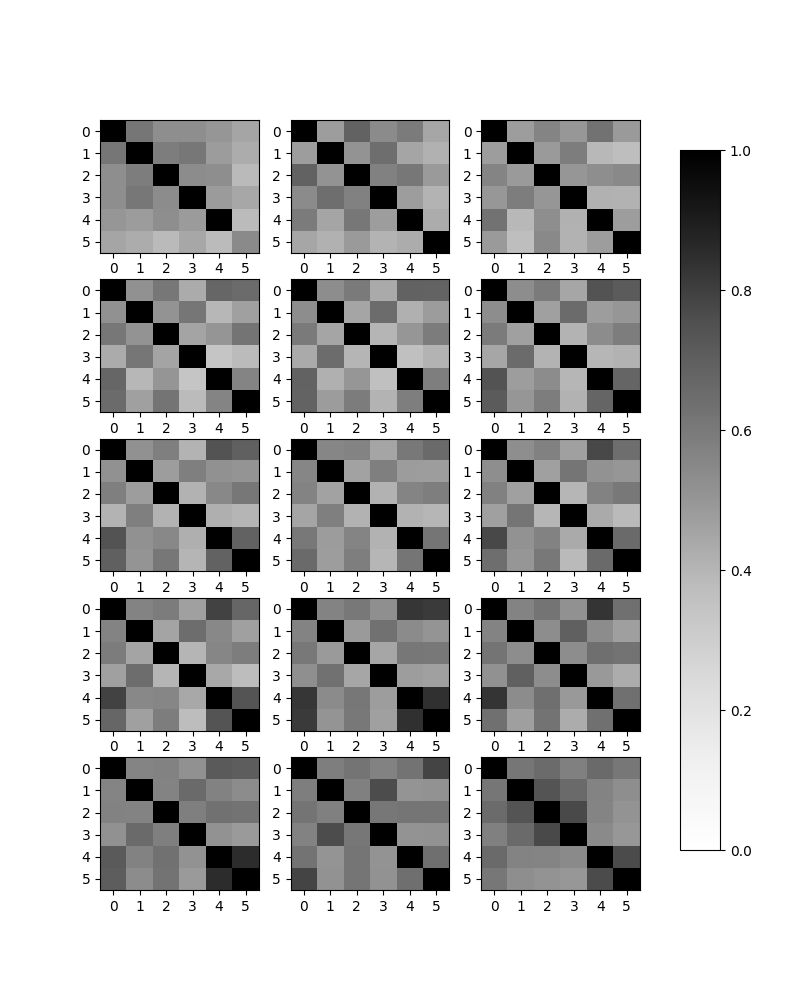
\includegraphics[width=\textwidth]{figs/f1.png}
		\caption[]%
		{{\small Second Fully Connected Layer}}    
		\label{fig:f1}
	\end{subfigure}
	\quad
	\begin{subfigure}[b]{0.475\textwidth}   
		\centering 
		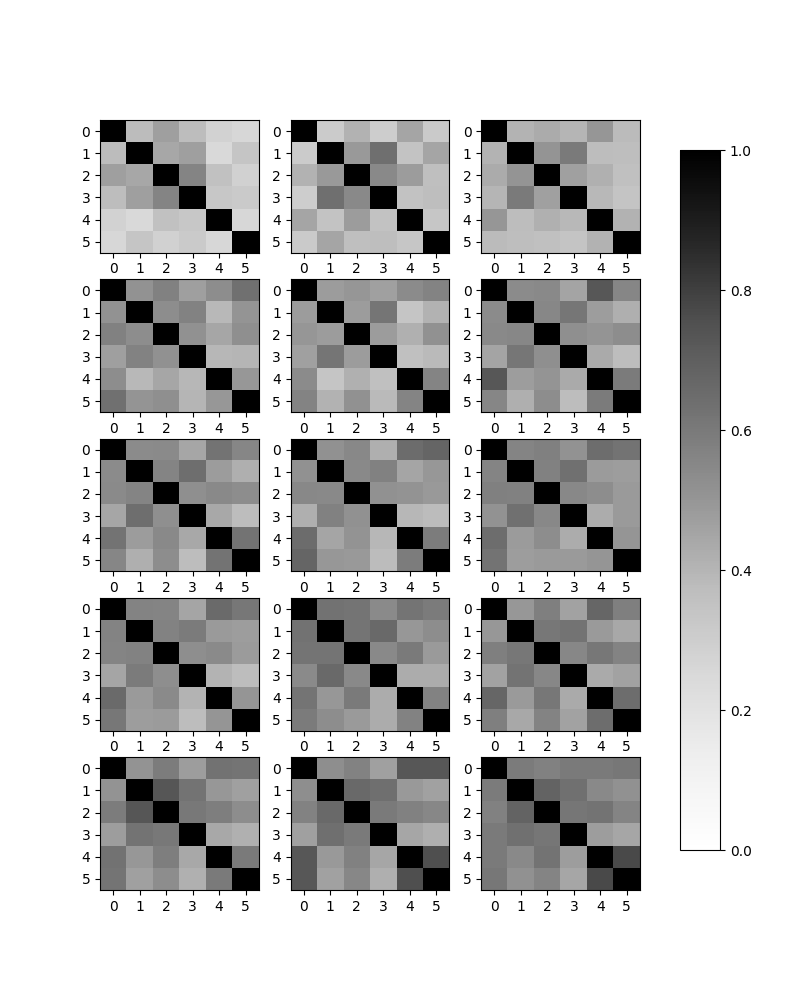
\includegraphics[width=\textwidth]{figs/output.png}
		\caption[]%
		{{\small Second Fully Connected Layer}}    
		\label{fig:output}
	\end{subfigure}
	\caption[]
	{\small The similarity matrices of 6 models for Epoch $1-10$,$20,30,40,50,100$} 
	\label{fig:model-comparison}
\end{figure*}

For the models we generate, \emph{NN0, NN1, NN4, NN5} has exactly the same structure but different initializations while \emph{NN2} and \emph{NN3} share the same structure. What's more, \emph{NN1} and \emph{NN3} have different learning rates and momentums. Having this similarity measurement, we start with looking at the model similarity at different epochs. More specifically, we generate similarity matrix for two convolution layers, two fully connected layers. As shown in Fig.~\ref{fig:model-comparison}, for all the 4 layers, from epoch to epoch, the \emph{NN0}, \emph{NN4} and \emph{NN5} become more and more similar to each other. We can also see that  \emph{NN2} and \emph{NN3} become more similar to each other but different from the other 4 neural networks in Fig.~\ref{fig:c1} and Fig.~\ref{fig:c2}.

In addition to model comparison, we could could also use our similarity algorithm for comparing different layers. Shown in Fig.~\ref{fig:layer-comparison},  we find out that two convolution layers tend to treat these samples in a similar way as well
as two fully connected layers. We guess the reason is that convolution layers may capture different features than linear layers.


\begin{figure*}
	\centering
	\begin{subfigure}[b]{0.3\textwidth}
		\centering
		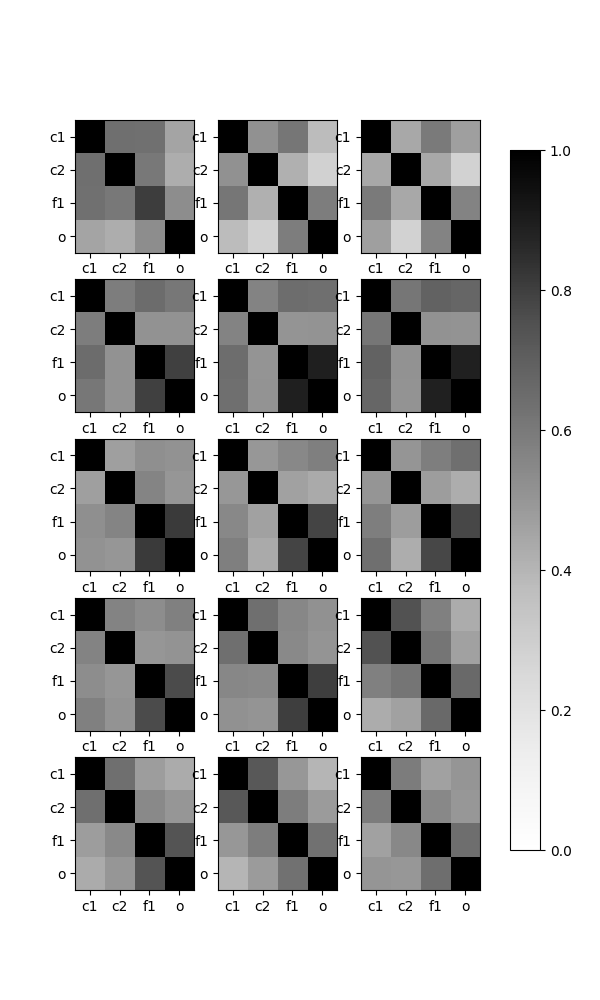
\includegraphics[width=\textwidth]{figs/nn1_sim.png}
		\caption[]%
		{{\small NN0}}    
		\label{fig:nn0}
	\end{subfigure}
	\hfill
	\begin{subfigure}[b]{0.3\textwidth}  
		\centering 
		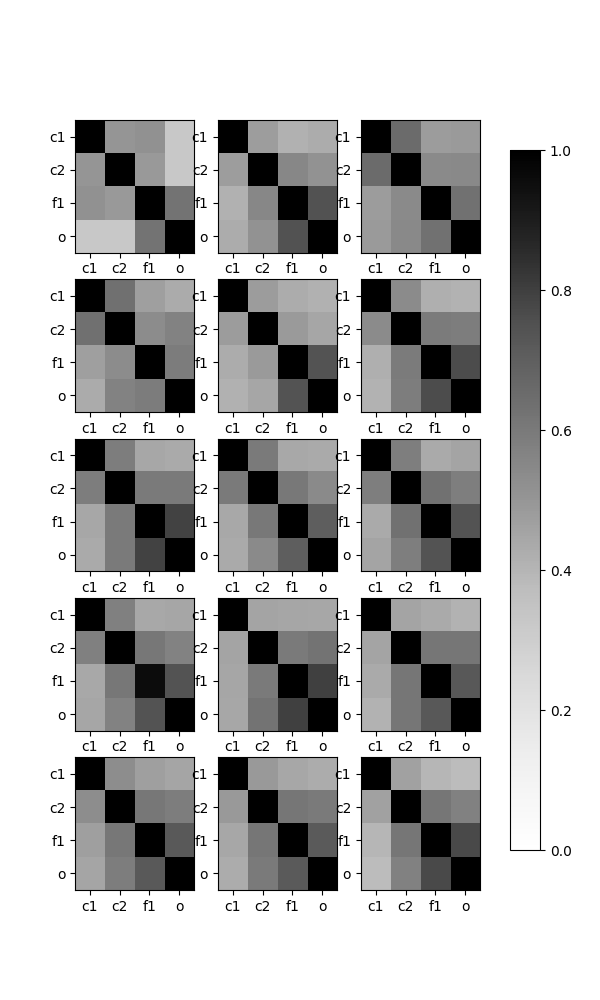
\includegraphics[width=\textwidth]{figs/nn2_sim.png}
		\caption[]%
		{{\small NN1}}    
		\label{fig:nn1}
	\end{subfigure}
	\hfill
	\begin{subfigure}[b]{0.3\textwidth}  
		\centering 
		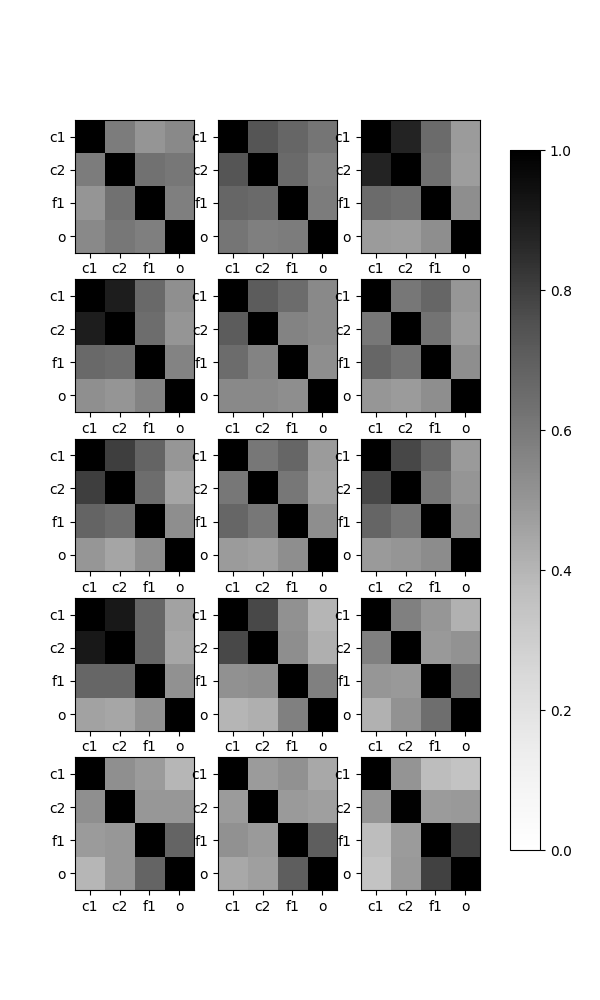
\includegraphics[width=\textwidth]{figs/nn3_sim.png}
		\caption[]%
		{{\small NN2}}    
		\label{fig:nn2}
	\end{subfigure}
	\vskip\baselineskip
	\begin{subfigure}[b]{0.3 \textwidth}   
		\centering 
		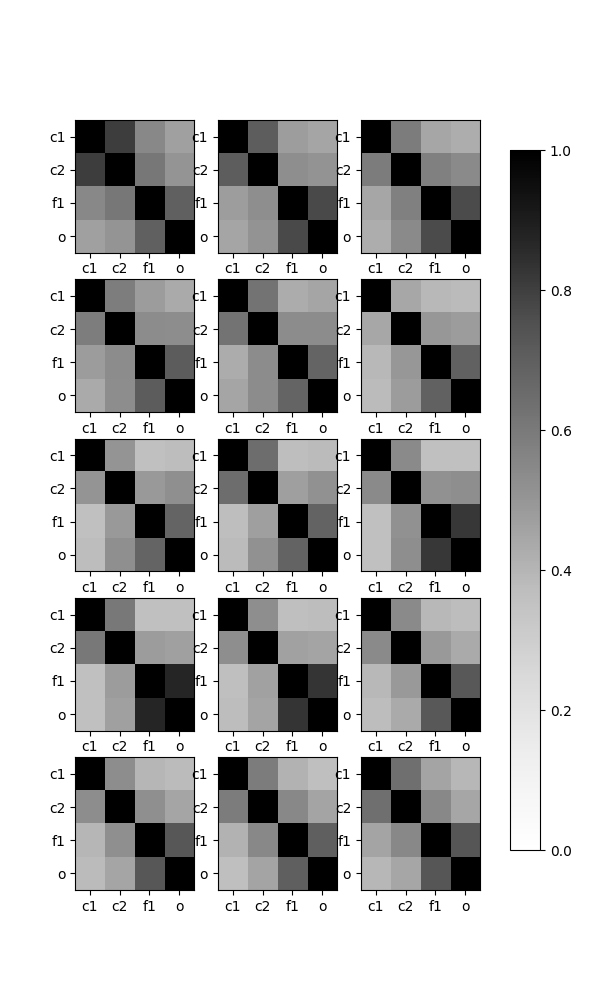
\includegraphics[width=\textwidth]{figs/nn4_sim.png}
		\caption[]%
		{{\small NN3}}    
		\label{fig:nn3}
	\end{subfigure}
	\hfill
	\begin{subfigure}[b]{0.3\textwidth}   
		\centering 
		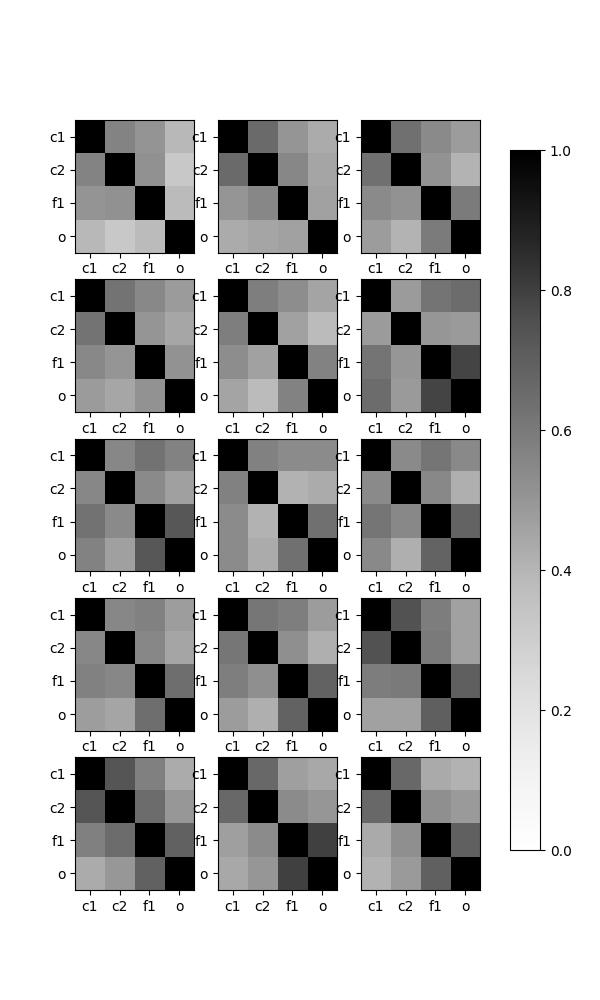
\includegraphics[width=\textwidth]{figs/nn5_sim.png}
		\caption[]%
		{{\small NN4}}    
		\label{fig:nn4}
	\end{subfigure}
	\hfill
	\begin{subfigure}[b]{0.3\textwidth}   
		\centering 
		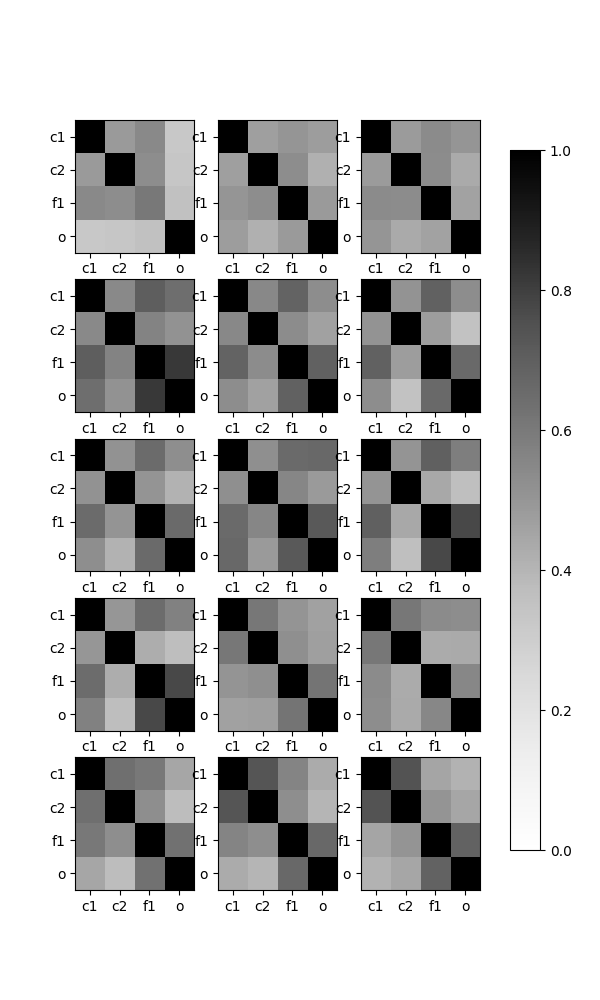
\includegraphics[width=\textwidth]{figs/nn6_sim.png}
		\caption[]%
		{{\small NN5}}    
		\label{fig:nn5}
	\end{subfigure}
		\caption[]
	{\small The similarity matrices of 4 layers for Epoch $1-10$,$20,30,40,50,100$} 
	\label{fig:layer-comparison}
\end{figure*}



\section{Conclusion}
In this project, we generate models from Fashion-MNIST datasert, collect the activation vectors of all the instances for all the models and propose a new way of comparing different neural networks. we could expect our clustering method could cluster the models such that within one cluster  two models recognize the instances more similarly than two models from two different clusters. And based on the distribution of the instances, we could summarize the behavior of the models in the same cluster.  We could also see the application of the method when comparing different layers. The core of our method based on the fact that similar models or models should have more similar activation responses to the dataset.

 
 \section{Future Work}
 Currently, our work only look at a epoch each time. The next step could be how to combine these vectors when comparing a pair of models. 
 This could give us a more comprehensive presentation of the data clusters. Moreover, we would like to apply our method to more samples and more models of more different structures to prove the scalability of our method. What's more, a better clustering method could be used other than K-means, For example, we could train a neural network to classify these activation vectors or using traditional method like multi-class SVM. We could also consider other dimension reduction method like TSNE or UMAP for better results. Finally, other measures of similarity of data clusterings could be included since the measurement we choose will have a direct effect on the cluster of models we generate.
 


\section{List 5 major publications that are most relevant to this project, and how they are related.}

\begin{itemize}
	
\item This survey conducted by Kriegel et. al.~\cite{Kriegel:2009:CHD:1497577.1497578} give a summary of several clustering methods for the high-dimension dataset.

\item t-distributed stochastic neighbor embedding(TSNE)~\cite{vanDerMaaten2008} proposed by Maaten et. al. is currently widely for dimension reduction.

\item Principal component analysis(PCA)~\cite{jolliffe86} is another widely used dimension reduction method.

\item Kernel density estimation~\cite{article} is a non-parametric way to estimate the probability density function of a random variable. We can make use it to estimate the distribution of instances for each model.

\item Recent work~\cite{article2,article3}  also propose different algorithms to do clustering for high-dimension and low sample size data.

 \end{itemize}



\bibliographystyle{plain}
%\bibliographystyle{abbrv-doi-narrow}
%\bibliographystyle{abbrv-doi-hyperref}
%\bibliographystyle{abbrv-doi-hyperref-narrow}

\bibliography{ref}
%\bibliographystyle{abbrv}
\end{document}
